\chapter{Resource Entitlement}


In many ways, a virtualized server is analogous to an apartment building. Several virtual machines are provisioned within a physical machine, just as several apartments are owned or rented in an apartment building. The hallways and other common spaces are compactly designed under the assumption that not all of the residents will use them at the same time. Similarly, in a virtualized system, the core hardware resources, including the CPU, memory, network bandwidth, and disk I/O are shared among virtual machines under the assumption that not all virtual machines will need these resources at the same time. Virtualization of the critical system resources leads to effective utilization of the hardware and improves cost-effectiveness. A sample virtualized system running heterogeneous applications is shown in Figure \ref{fig:resourceutil} to represent the soul of higher utilization. The virtual machines, each which would have under-utilized the host's CPU, effectively share the CPU in a virtualized environment, leading to higher utilization.  

\begin{figure}[htbp]
\centering
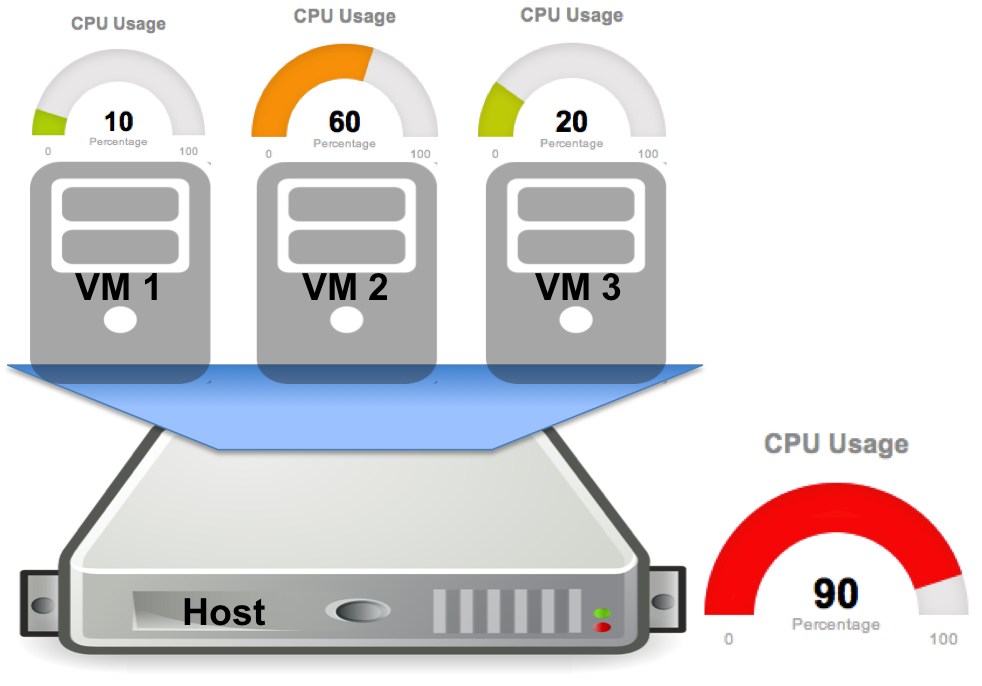
\includegraphics[width=130mm]{resourceutil.png}
\caption{Virtualization - CPU Utilization Perspective}
\label{fig:resourceutil}
\end{figure}

Drawing from our analogy, every apartment in the apartment building expects a certain degree of privacy and isolation. The presence of over-consuming or noisy neighbors negatively impacts the peace and harmony of the building. Similarly, every virtual machine requires a degree of isolation from other virtual machines in order to fulfill its own service requirements. For example, consider a system in which four physical CPUs are shared among four virtual machines. If one of the virtual machines tries to utilize all four CPUs accessible to it, the other virtual machines begin to starve, even though they hold other resources, such as memory, network, and disk I/O. Such situations must be avoided, and individual machines must be guaranteed their minimum entitled share of the resources at all times. This chapter analyzes the default isolation effectiveness provided by the representative virtualization solutions and also describes the available resource entitlement mechanisms that can be used.


To evaluate the resource isolation efficiency of KVM, Xen, and Linux Containers, we measure the impact of an over-stressed virtual machine on other virtual machines running on the same host. We created two identical virtual machines on each of the physical servers, sharing all of the host's resources between them, and then measured the change in execution times of the sample applications (w1, w2, w3, and w4) running on one virtual machine when stress was created on the other virtual machine using \emph{stress} \cite{stress} tool.
\begin{figure}[H]
        \centering
        \begin{subfigure}[b]{0.99\textwidth}
                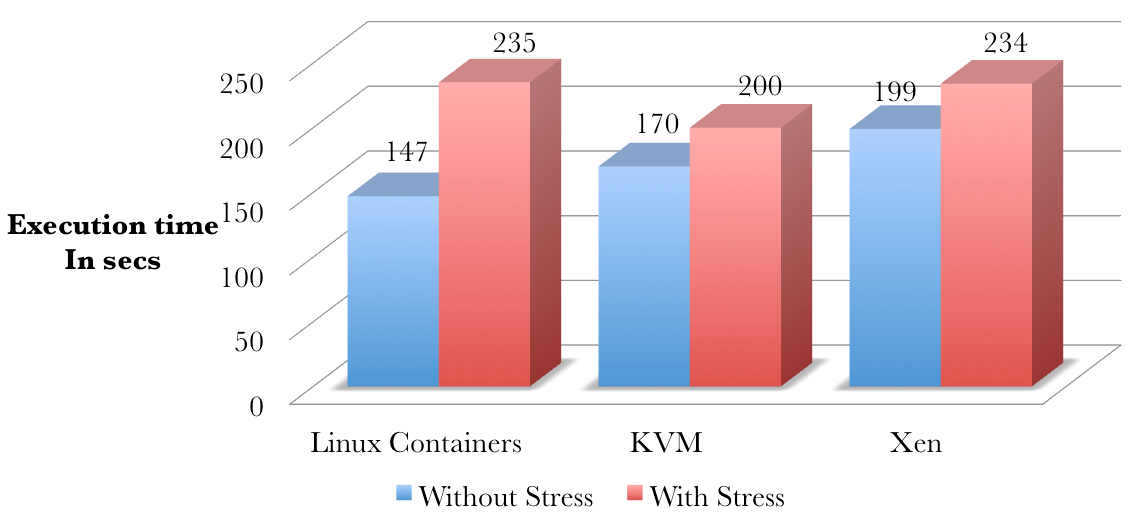
\includegraphics[width=\textwidth]{cpustress.png}
                \caption{Impact of stress on sample application w1}
                \label{fig:cpustress1}
        \end{subfigure}%
        ~ %add desired spacing between images, e. g. ~, \quad, \qquad etc.
        \qquad \newline %\hspace{8 mm} 
          %(or a blank line to force the subfigure onto a new line)
        \begin{subfigure}[b]{0.8\textwidth}
                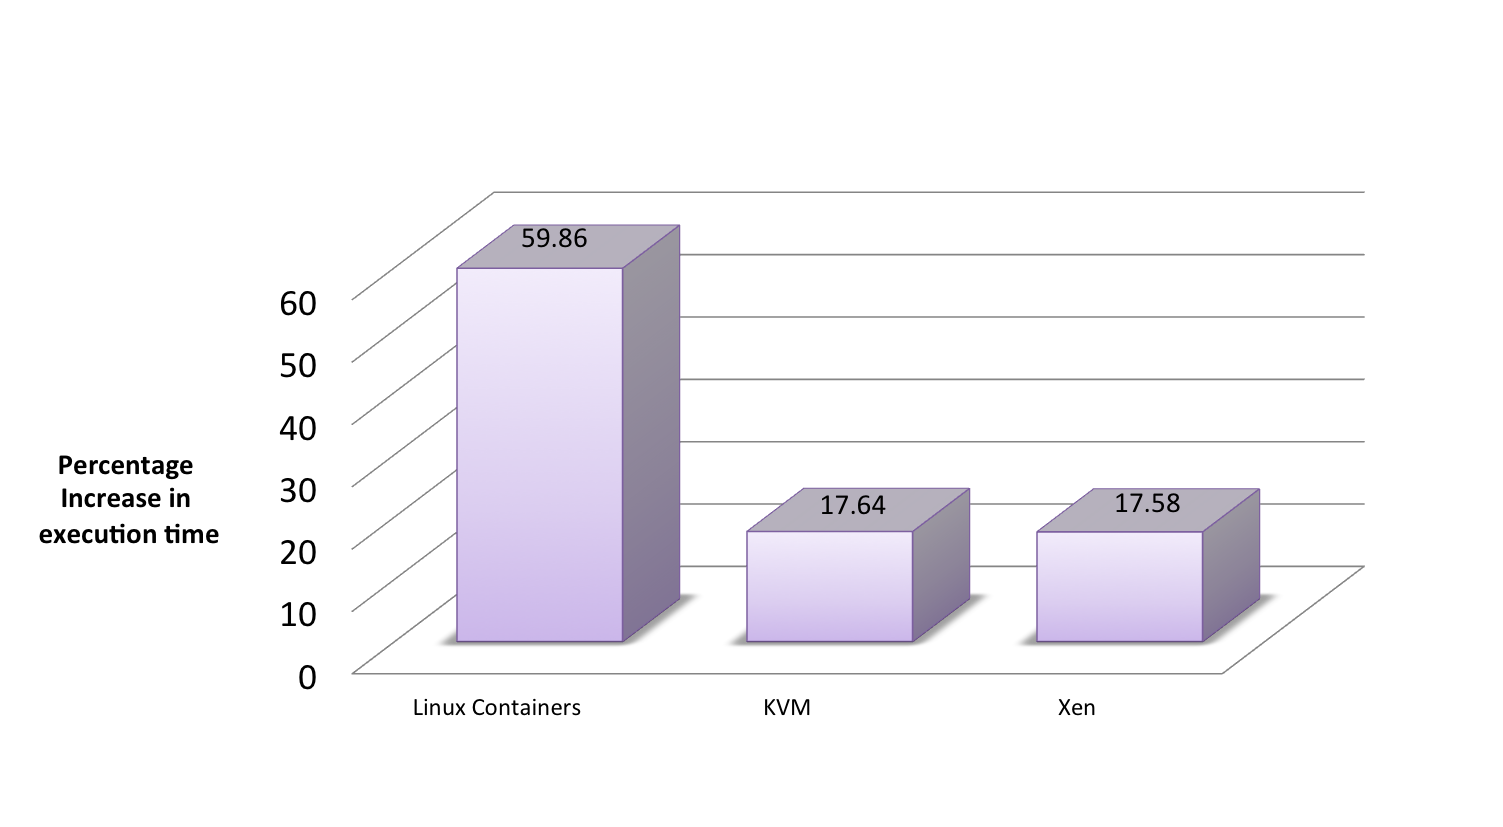
\includegraphics[width=\textwidth]{cpustressp.png}
                \caption{Impact of stress in percentage increase}
                \label{fig:cpustressp}
        \end{subfigure}
        \caption{CPU Isolation Efficiency}\label{fig:cpuisolation}
\end{figure}

Figure \ref{fig:cpustress1} summarizes the change in execution time of the sample application w1 (performing CPU intensive tasks) on each of the virtualization platforms. The x-axis represents the virtualization platforms, and the y-axis represents execution time, both before and after stress was applied. Based on the results shown in Figure \ref{fig:cpustress1}, the percentage increase in execution times was calculated for each platform and summarized in Figure \ref{fig:cpustressp}. The percentage increase in execution time is inversely proportional to the CPU isolation efficiency offered by the virtualization platform. In other words, in an effectively isolated environment, the increase in execution time would be minimal. Hence, it is evident from the results that KVM and Xen offer superior CPU isolation for the virtual machines, while Linux Containers are poorly isolated with respect to CPU.

\begin{figure}[H]
        \centering
        \begin{subfigure}[b]{0.99\textwidth}
                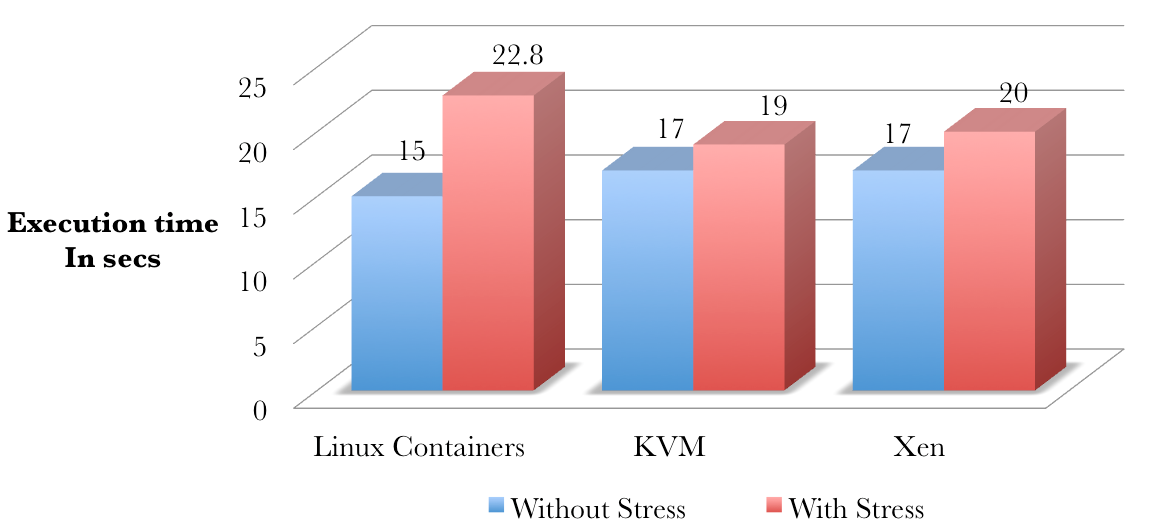
\includegraphics[width=\textwidth]{memstress.png}
                \caption{Impact of stress on sample application w2}
                \label{fig:memstress1}
        \end{subfigure}%
        ~ %add desired spacing between images, e. g. ~, \quad, \qquad etc.
        \qquad \newline %\hspace{8 mm} 
          %(or a blank line to force the subfigure onto a new line)
        \begin{subfigure}[b]{0.8\textwidth}
                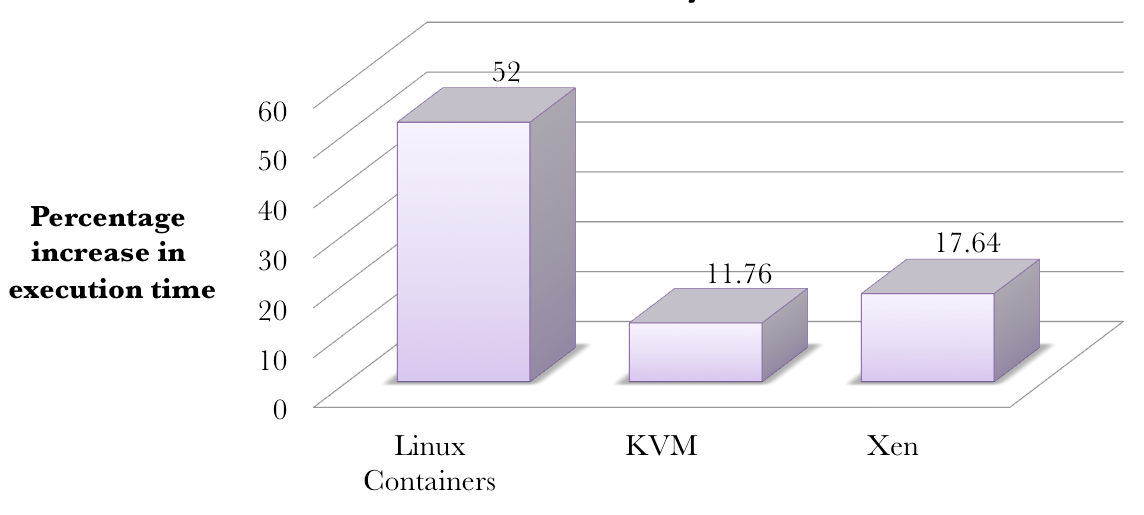
\includegraphics[width=\textwidth]{memstressp.png}
                \caption{Impact of stress in percentage increase}
                \label{fig:memstressp}
        \end{subfigure}
        \caption{Memory Isolation Efficiency}\label{fig:memisolation}
\end{figure}

Figure \ref{fig:memstress1} summarizes the change in execution time of the sample application w2 (performing memory intensive tasks) on each of the virtualization platforms. The x-axis represents the virtualization platforms, and the y-axis represents execution time, both before and after stress was applied. Based on the results shown in Figure \ref{fig:memstress1}, the percentage increase in execution time was calculated for each platform and summarized in Figure \ref{fig:memstressp}. The percentage increase in execution time is inversely proportional to the memory isolation efficiency offered by the virtualization platform. In other words, in an effectively isolated environment, the increase in execution time wwould be minimal. It is evident from the results that KVM offers superior memory isolation for the virtual machines, while Linux Containers are poorly isolated with respected to memory.

\begin{figure}[H]
        \centering
        \begin{subfigure}[b]{0.99\textwidth}
                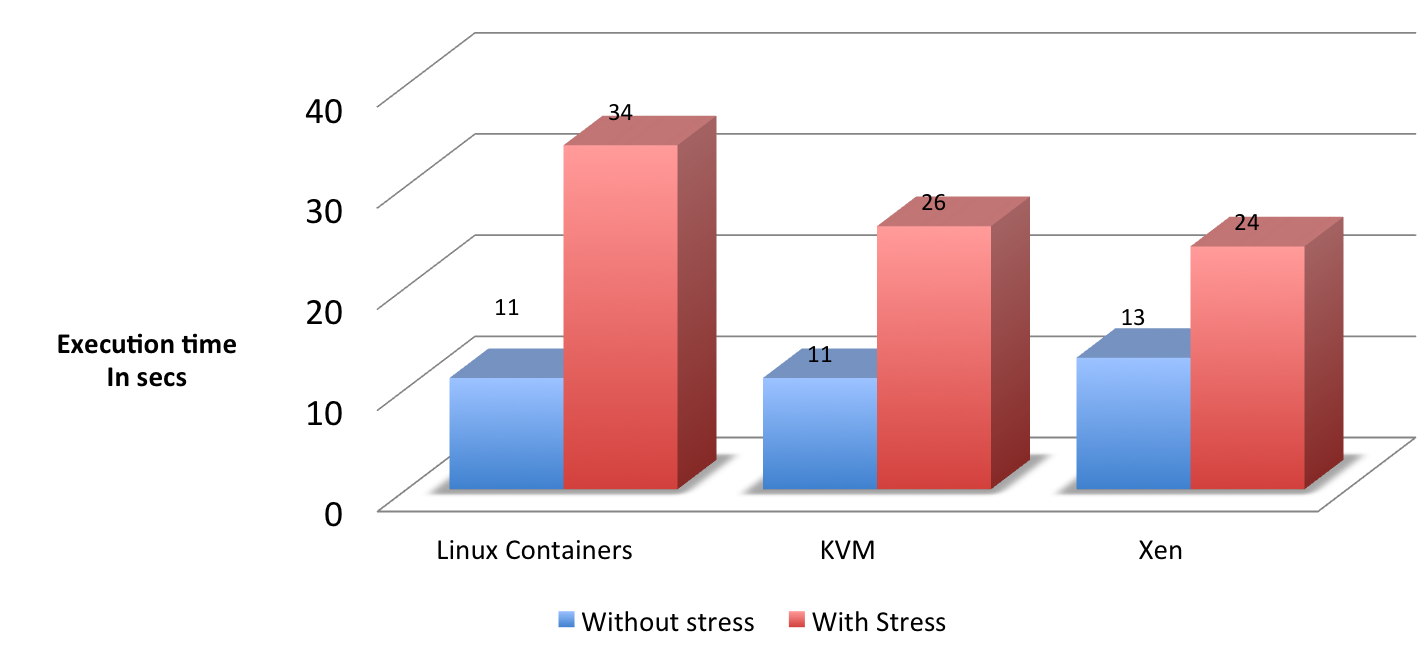
\includegraphics[width=\textwidth]{netstress.png}
                \caption{Impact of stress on sample application w3}
                \label{fig:netstress1}
        \end{subfigure}%
        ~ %add desired spacing between images, e. g. ~, \quad, \qquad etc.
        \qquad \newline %\hspace{8 mm} 
          %(or a blank line to force the subfigure onto a new line)
        \begin{subfigure}[b]{0.8\textwidth}
                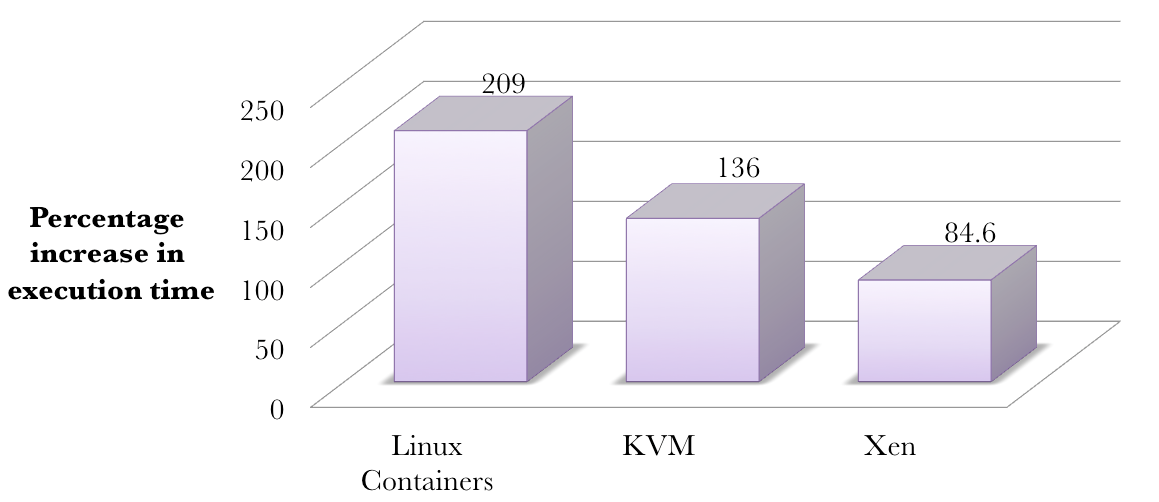
\includegraphics[width=\textwidth]{netstressp.png}
                \caption{Impact of stress in percentage increase}
                \label{fig:netstressp}
        \end{subfigure}
        \caption{Network Isolation Efficiency}\label{fig:netisolation}
\end{figure}

Figure \ref{fig:netstress1} summarizes the change in execution time of the sample application w2 (performing network I/O operations) on each of the virtualization platforms. The x-axis represents the virtualization platforms, and the y-axis represents execution time, both before and after stress was applied. Based on the results shown in Figure \ref{fig:netstress1}, the percentage increase in execution times was calculated for each platform and summarized in Figure \ref{fig:netstressp}. The percentage increase in execution time is inversely proportional to the isolation efficiency of network I/O operations offered by the virtualization platform. In an effectively isolated environment, the increase in execution time would be minimal. It is evident from the results that Xen offers superior network isolation for the virtual machines, while Linux Containers are poorly isolated with respected to network bandwidth.


\begin{figure}[H]
        \centering
        \begin{subfigure}[b]{0.99\textwidth}
                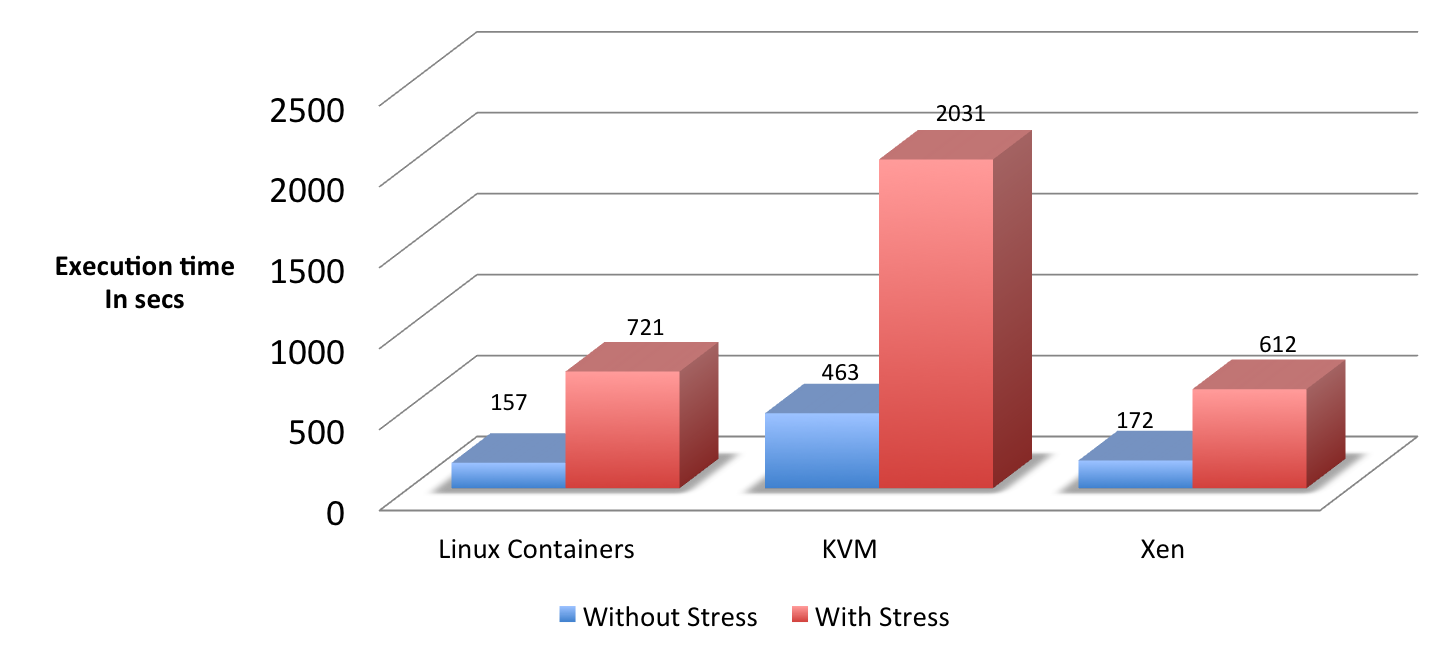
\includegraphics[width=\textwidth]{diskstress.png}
                \caption{Impact of stress on sample application w4}
                \label{fig:diskstress1}
        \end{subfigure}%
        ~ %add desired spacing between images, e. g. ~, \quad, \qquad etc.
        \qquad \newline %\hspace{8 mm} 
          %(or a blank line to force the subfigure onto a new line)
        \begin{subfigure}[b]{0.8\textwidth}
                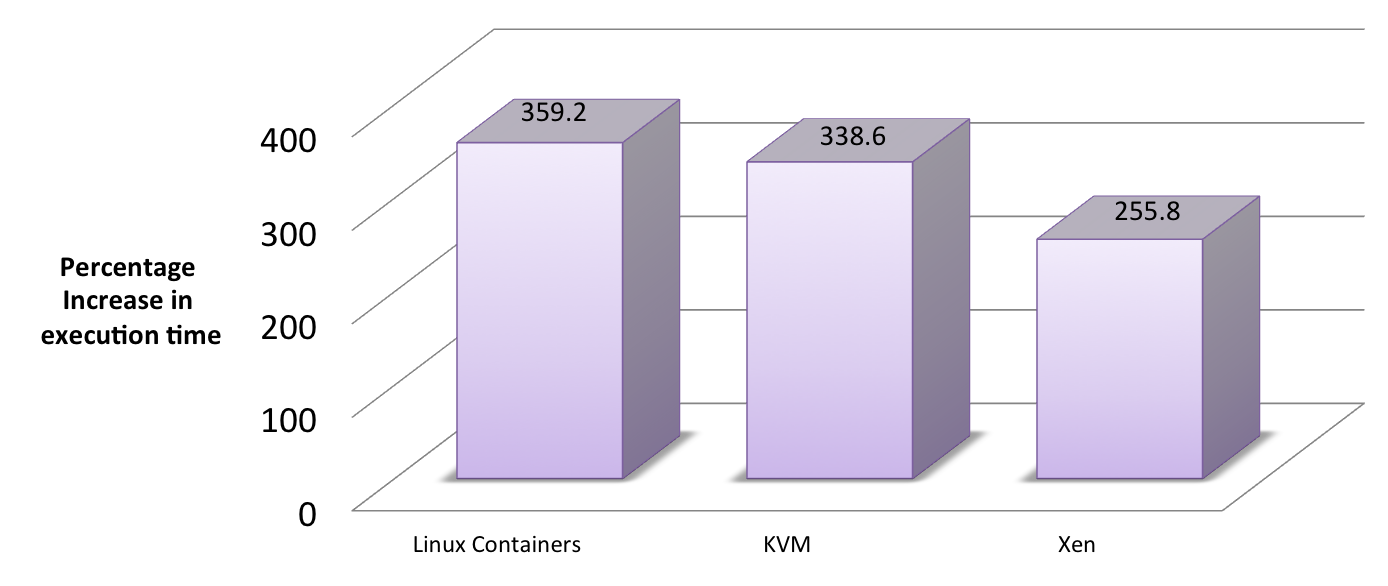
\includegraphics[width=\textwidth]{diskstressp.png}
                \caption{Impact of stress in percentage increase}
                \label{fig:diskstressp}
        \end{subfigure}
        \caption{Disk I/O Isolation Efficiency}\label{fig:diskisolation}
\end{figure}

Figure \ref{fig:diskstress1} summarizes the change in execution time of the sample application w4 (performing large number of disk I/O operations) on each of the virtualization platforms. The x-axis represents the virtualization platforms, and the y-axis represents execution time, both before and after stress was applied. Based on the results shown in Figure \ref{fig:diskstress1}, the percentage increase in execution times was calculated for each platform and summarized in Figure \ref{fig:diskstressp}. The percentage increase in execution time is inversely proportional to the  efficiency of isolation for disk I/O operations offered by the virtualization platform. In an effectively isolated environment, the increase in execution time would be minimal. It is evident from the results that Xen offers superior isolation for disk I/O operations for the virtual machines, while Linux containers and KVM provides poor isolation with respect to disk I/O operations.


%To test the resource isolation efficiency of KVM, Xen and Linux Containers by creating the ``noisy neighbor'' scenario, we created two virtual machines on each of the virtualized servers, sharing all the physical resources between them. We observed the impact on the performance of one virtual machine while stressing the other virtual machine to use as much resources it can. We used the stress \cite{stress} tool to create the load on CPU, memory, network and disk I/O. The Figure shows the change in execution times of the sample applications we had created for the overhead tests, before and after the stress was created on the second virtual machine.
%
%\begin{figure}[htbp]
%\centering
%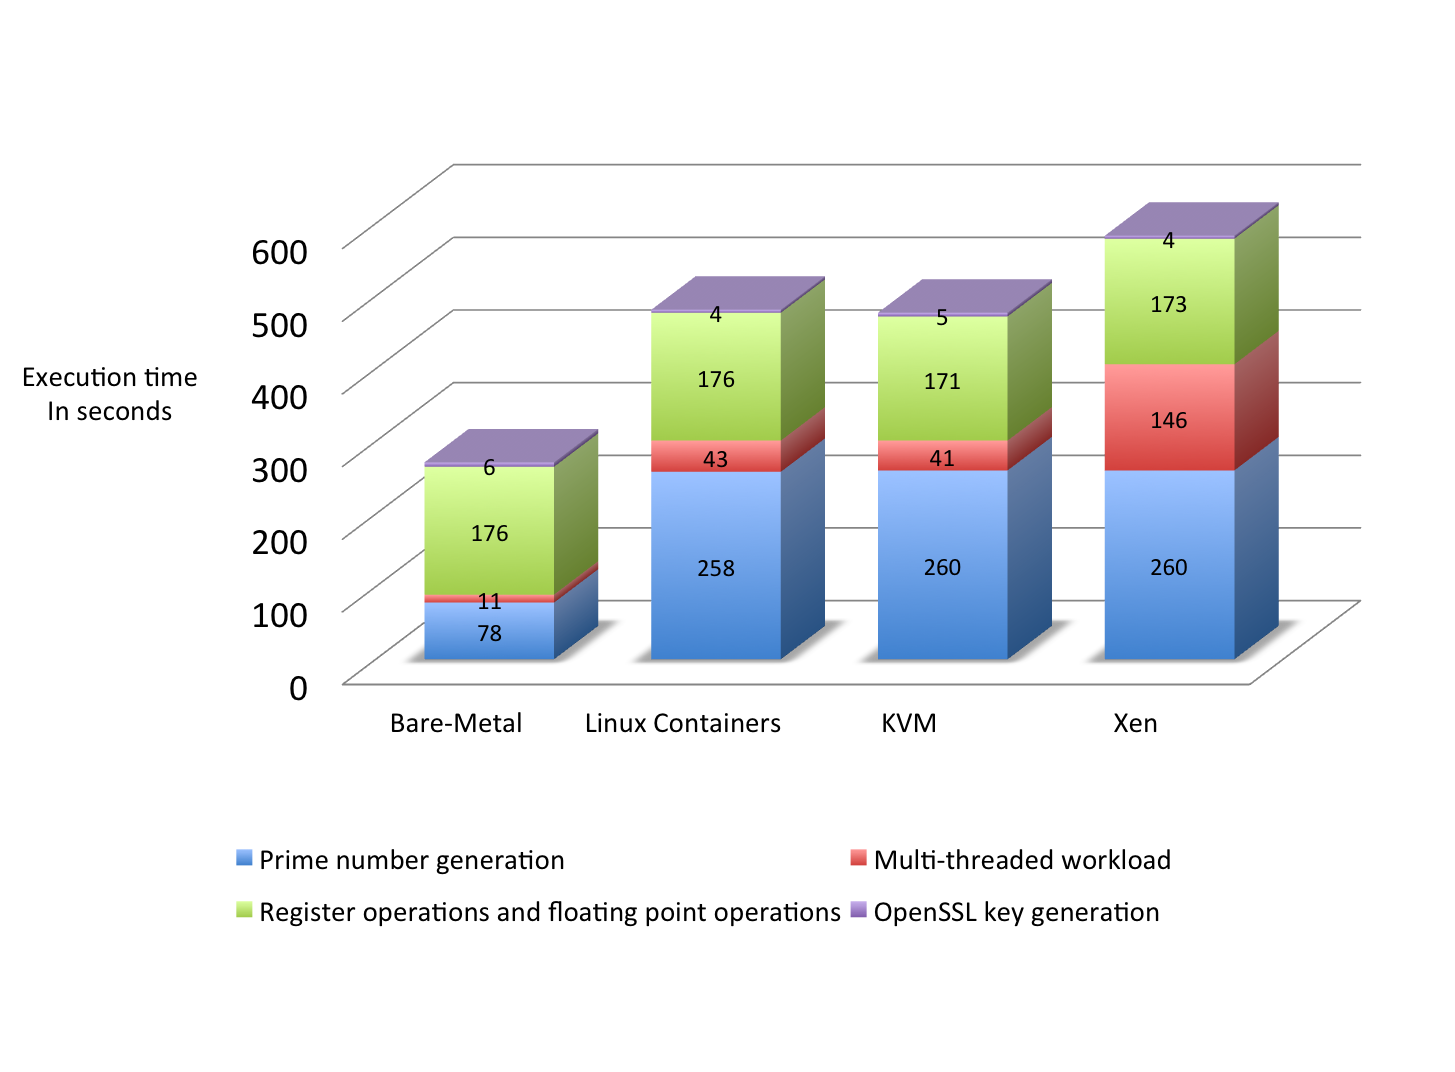
\includegraphics[width=130mm]{1cpu.png}
%\caption{CPU Isolation}
%\label{fig:cpustress}
%\end{figure}
%
%\begin{figure}[htbp]
%\centering
%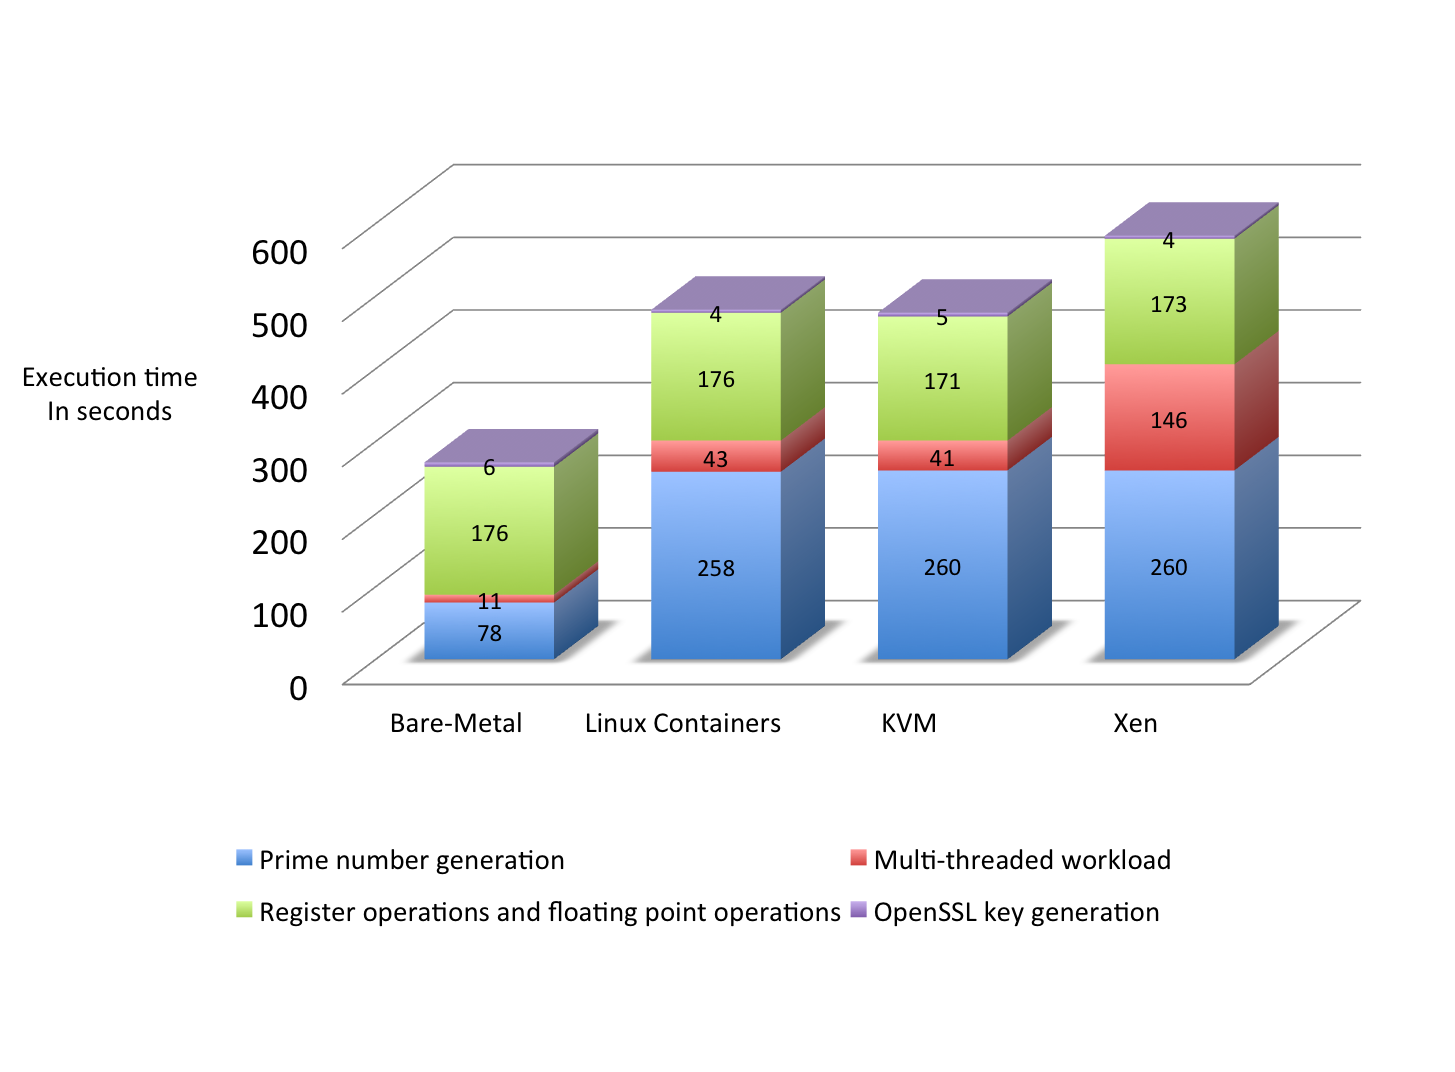
\includegraphics[width=130mm]{1cpu.png}
%\caption{Memory Isolation}
%\label{fig:memstress}
%\end{figure}
%
%\begin{figure}[htbp]
%\centering
%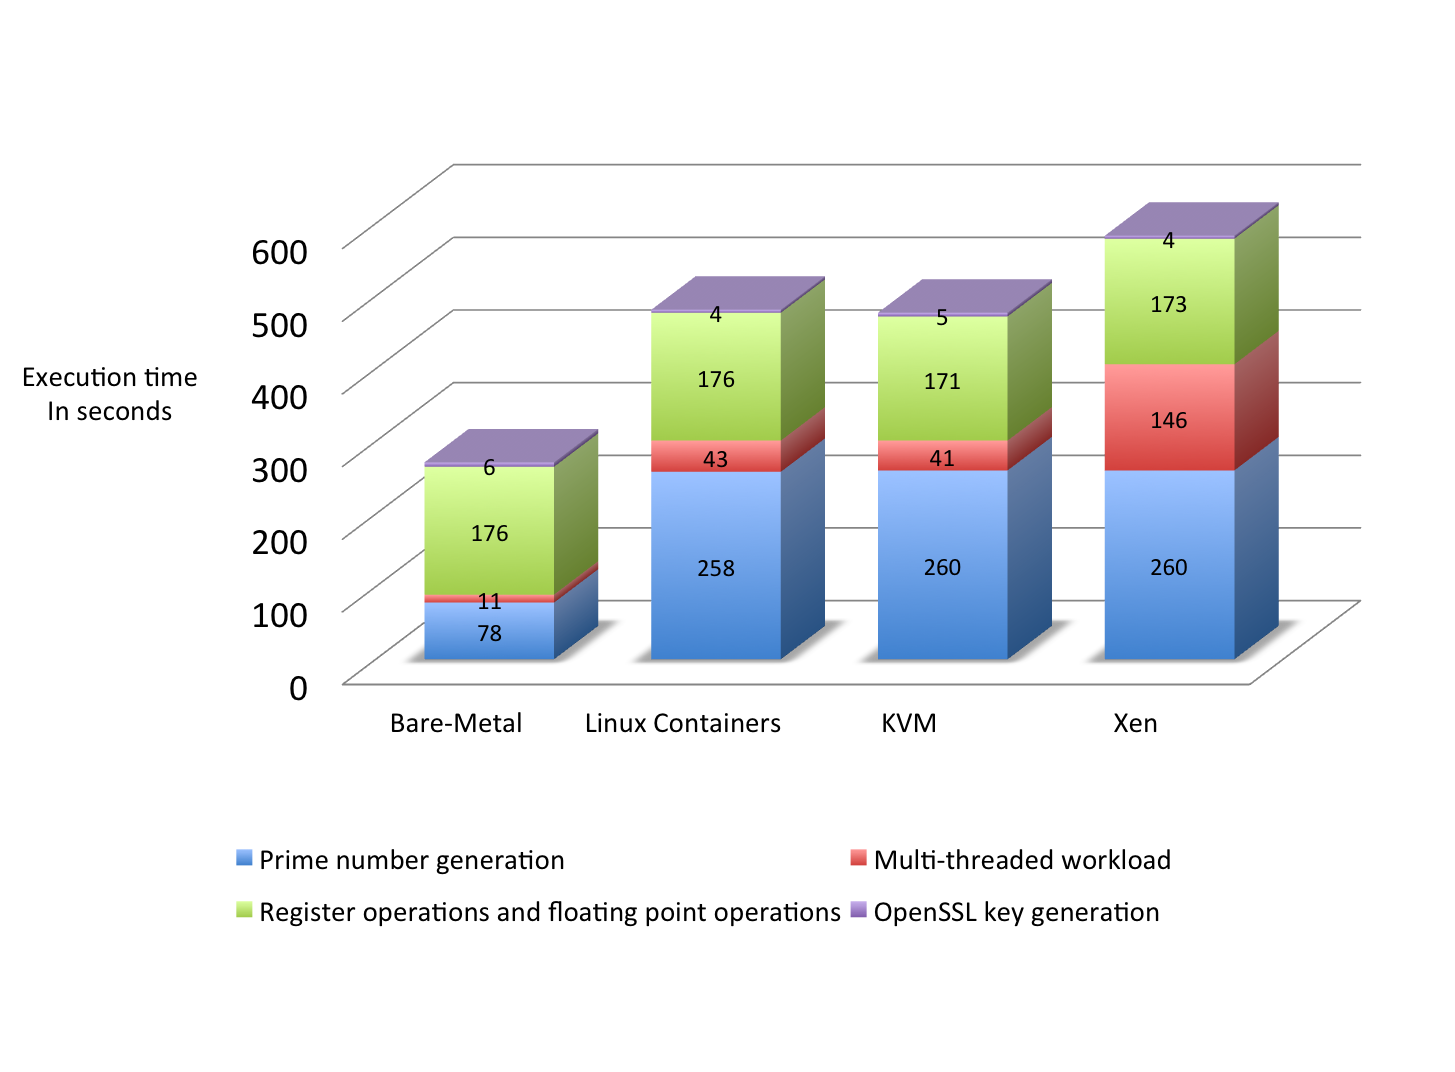
\includegraphics[width=130mm]{1cpu.png}
%\caption{Network Isolation}
%\label{fig:netstress}
%\end{figure}
%
%\begin{figure}[htbp]
%\centering
%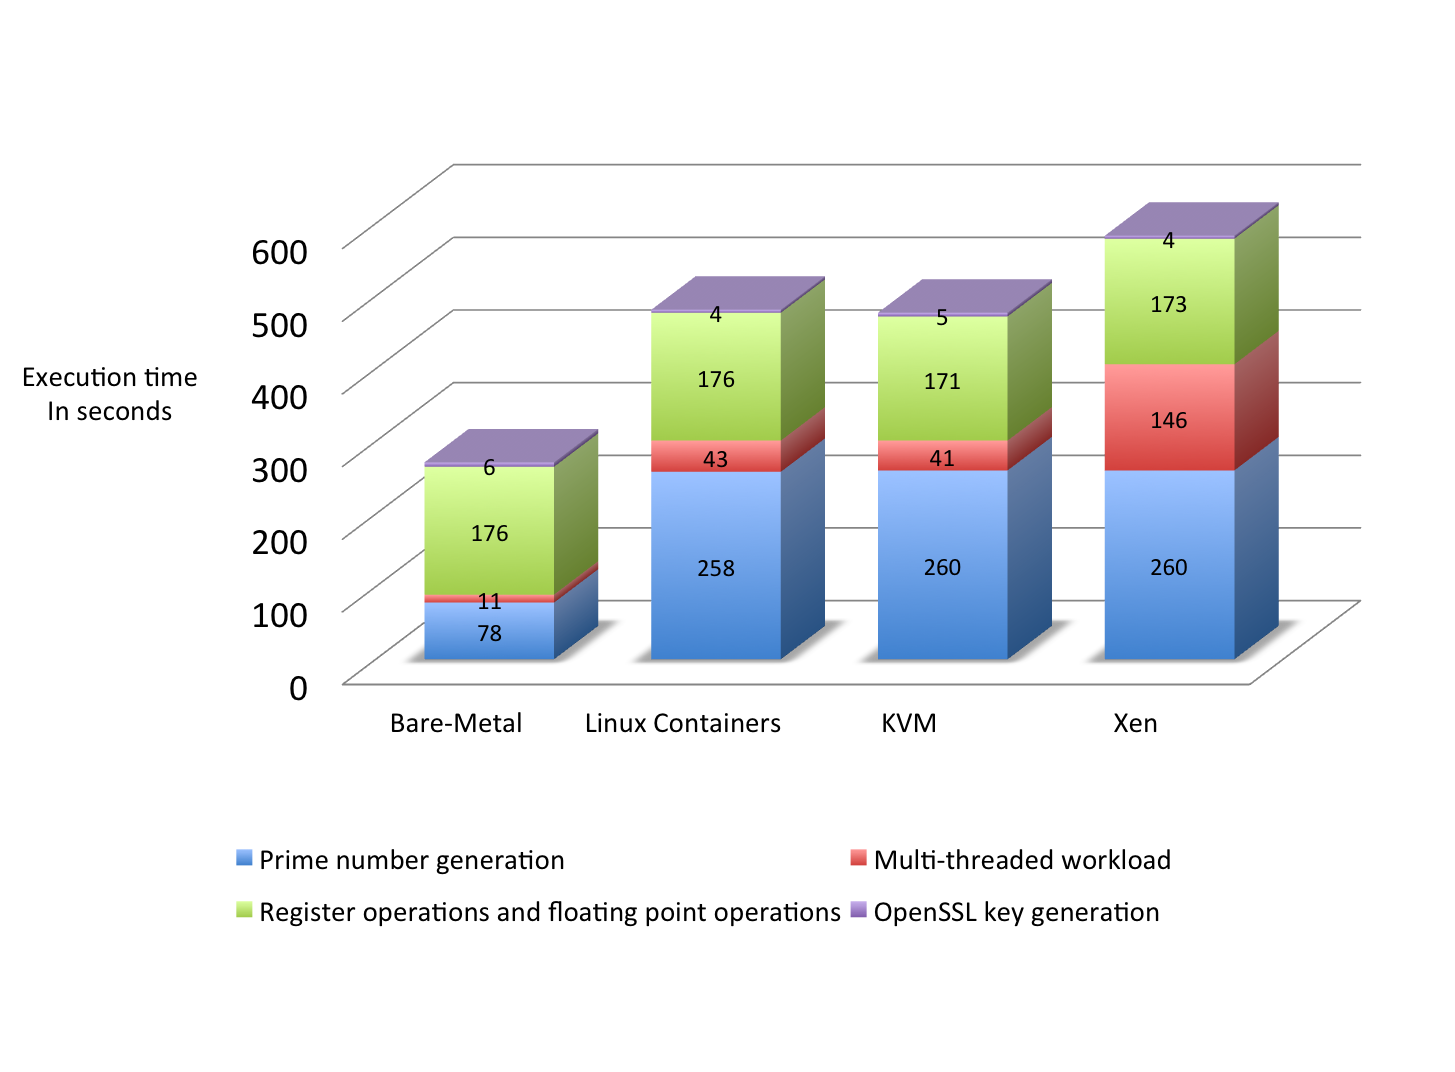
\includegraphics[width=130mm]{1cpu.png}
%\caption{Disk I/O Isolation}
%\label{fig:diskstress}
%\end{figure}



The results summarized in Figures \ref{fig:cpuisolation}, \ref{fig:memisolation}, \ref{fig:netisolation}, and \ref{fig:diskisolation} shows that none of KVM, Xen, and Linux Containers provide effective resource isolation, as stress applied on one virtual machine severely affected the performance of the application running on the other virtual machine. This lack of isolation would translate into unpredictable performance of applications running in virtualized infrastructure. The rest of this chapter addresses this issue by describing the facilities available to define limits and assure virtual machines of their entitlement in terms of CPU, memory, network bandwidth, and disk I/O. These facilities are applicable for all the virtualization platforms.





%sharing all the available resources among the virtual machines without any reservations or priorities yields unpredictable performance.The following section describes the facilities available in a Linux system, and the hypervisors to define limits and assure virtual machines of their entitlement in terms of CPU, memory, network bandwidth and disk I/O.

%The charts, \ref{fig:cpustress}, \ref{fig:memstress}, \ref{fig:netstress}, and \ref{fig:diskstress} shows that sharing all the available resources without any reservations or priorities among the virtual machines is not the configuration to have for ideal performance. The following sections describe the facilities available in the linux ecosystem, and the hypervisors to define limits and assure the virtual machines, of their entitlement in terms of CPU, memory, network bandwidth and disk I/O.  


Before considering the mechanisms to configure dedicated system resources for virtual machines, it is important to analyze and understand the nature of the workloads that the virtual machine will run. This information is helpful in two regards:
\begin{enumerate}
\item Prior knowledge of the workloads can be used in deciding which virtual machines to provision on the same server. For example, a virtual machine that runs a web server (i.e, using  more network and memory resources), and a virtual machine that runs a reporting application (i.e, with more disk I/O) are both ideal candidates to be virtualized on the same physical server, as they utilize different types of resources. On the other hand, running many virtual machines executing database workloads on the same physical machine would not be a good practice, as they would contend for the same types of resources.
\item The characteristics of the application can be used in deciding which resources to dedicate and which resources to share.
\end{enumerate}
Planning the resource policies for CPU and memory resources goes hand in hand, as the primary rule of thumb in achieving better performance is to feed the processors with data as fast as possible by keeping the data in memory regions closest to them. To plan the CPU and memory resource allocations, it is important to understand their architecture in the physical server. All modern server class hardware is equipped with multi-core processors architected to efficiently scale by distributing system memory near the individual CPUs. This configuration is known as \textit{Non-Uniform Memory Access(NUMA)}. 
\begin{figure}[H]
\centering
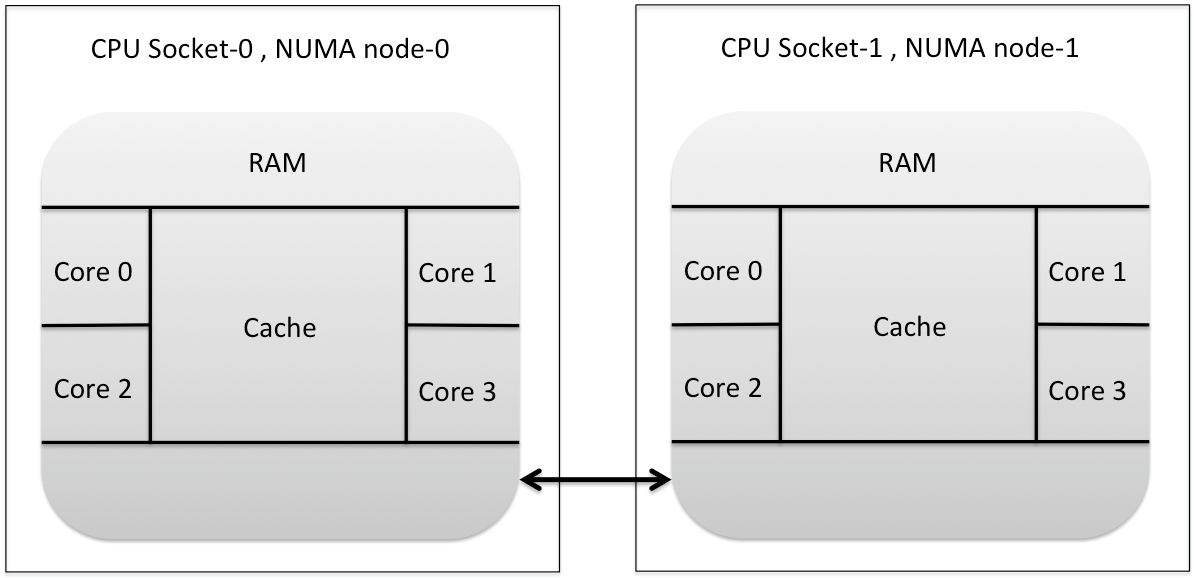
\includegraphics[width=130mm]{numa.png}
\caption{Hex-core CPU configuration (2 sockets, 2 node NUMA) }
\label{fig:numa}
\end{figure}
Figure \ref{fig:numa} shows a block diagram of a hex-core physical server in a 2-node NUMA configuration. CPU Socket-0 and CPU Socket-1 consist of two physical CPUs, each holding four processing cores. All four processing cores in each CPU-Socket share a common L3 cache memory. The memory on NUMA node-0 can be accessed faster by the processing cores contained in the CPU Socket-0. The memory on NUMA node-1 can be accessed faster by the processing cores contained in CPU Socket-1.


Memory access across NUMA nodes will be relatively slow (e.g., a processing core in CPU Socket-0 accessing memory in NUMA node-1), and does not make efficient use of the L3 cache. This level of architectural information about the CPU and the memory hardware can be obtained using the following commands: \\
\begin{itemize}
\item \textbf{lscpu} \cite{lscpu} - Used to gather CPU architecture information from sysfs and /proc/cpuinfo
\item \textbf{numactl --hardware }\cite{numactl} - Used to display inventory of available nodes on the system. 
\end{itemize}


While analyzing the workloads with respect to CPU and memory entitlements, it is important to identify whether the application is multi-threaded. If yes, we must check if multiple threads doing independent CPU-intensive tasks or are dependent on each other and shared memory resources. By default, the Linux scheduler tries to keep all CPUs busy by moving tasks from overloaded CPUs to idle CPUs. This may be detrimental to the performance of the VMs on NUMA-based hardware, as a guest cannot take advantage of its accumulated state in the processor, including the instructions and data in the local cache \cite{procaffinity}. If the applications are single-threaded, the CPU reservations can be straightforward; ``pinning'', or assigning an ``affinity'' to the CPU, binding it to a physical CPU core will improve the performance of the application running on the virtual machine. CPU pinning or setting an affinity refers to assigning a specific process or virtual machine to a particular CPU core, such that the virtual machine is always scheduled (only) on that particular CPU core. In a carefully planned system, if all virtual machines are limited to appropriate set(s) of CPU cores, the virtual machines can run on their dedicated cores with little interruption, leading to improved performance. It is also useful to note that, access to an additional CPU core that may be shared across the system would help in alleviating interruptions by offloading threads performing operating system maintenance activities.

If the workload is multi-threaded, and the threads are performing mostly independent CPU-intensive tasks, the ideal policy would be to distribute them across as many processing cores as possible. This will improve parallelism, and hence improve performance. On the other hand, pinning virtual machines running multiple CPU-intensive threads to a single processing core would result in sub-optimal performance. If the workload is multi-threaded, and the threads are performing memory-intensive tasks with shared resources, the ideal policy would be to make sure they are scheduled on the same NUMA node, so that they can utilize multiple processing cores, yet share the local cache memory efficiently. CPU pinning and NUMA assignment can be implemented using the following Linux commands. 
\begin{itemize}
\item\textbf{ Taskset }\cite{taskset} - Used to retrieve the CPU affinity of a running process given its PID, or to launch a new command with a given CPU affinity. \\
Example: \texttt{taskset -c 0,2,4 kvmtest1} \\
pins the kvmtest1 process to the cores, 0, 2, and 4.
\item \textbf{Numactl} \cite{numactl} - Used to confine a process to a NUMA node, i.e, multiple cores sharing the same L3 cache. This helps to prevent virtual machines from being scheduled across NUMA pools.\\
Example:\texttt{ numactl --cpunodebind=0 --membind=0 kvmtest1 }\\
binds the guest kvmtest1 to the first CPU Socket, and also restricts memory use to the associated NUMA pool.
\end{itemize}
Though CPU pinning and NUMA node assignment limit virtual machines to confined resource pools, it may be impractical to use these mechanism in situations where the number of virtual machines is much greater than the number of processing cores. In such scenarios, a granular resource management mechanism, cgroups(control groups) (discussed in chapter 3) work well. cgroups are a Linux kernel feature that allows limiting and accounting of resources at a granular level. cgroups enable administrators to assign relative CPU shares to the virtual machines, indicating their priorities when accessing CPU resources, while still obeying the policies set by taskset and numactl.


The easiest method to achieve network isolation among virtual machines is to dedicate individual network interface hardware on the host to each virtual machine. This method is often justified by the relatively low cost of network interface cards. In situations where network bandwidth needs to be shared among virtual machines, cgroups can be used to classify the virtual machines into groups and dynamically assign priorities to them.

 
Implementing entitlement policies for disk I/O operations is relatively simpler. In most cases, a physical server contains several hardware adapters for the locally attached storage or block devices, each dedicated to a virtual machine. The disk I/O operations that a virtual machine performs can be specifically rate-limited for reads/write operations by individual processes using cgroup hierarchies. The blkio subsystem of cgroups enables throttling and accounting of I/O operations across the linux I/O scheduler. On a performance note, virtual machines tend to perform better with the deadline I/O scheduler with the ``nocache'' option, than the default CFQ I/O scheduler due to the avoidance of double caching.
 
%this chapter, we evaluate our system on the basis of reliability, scalability, and network longevity.
%
%\section{Reliability}\label{sec:reliability}
%
%\begin{figure}[htbp]
%\centering
%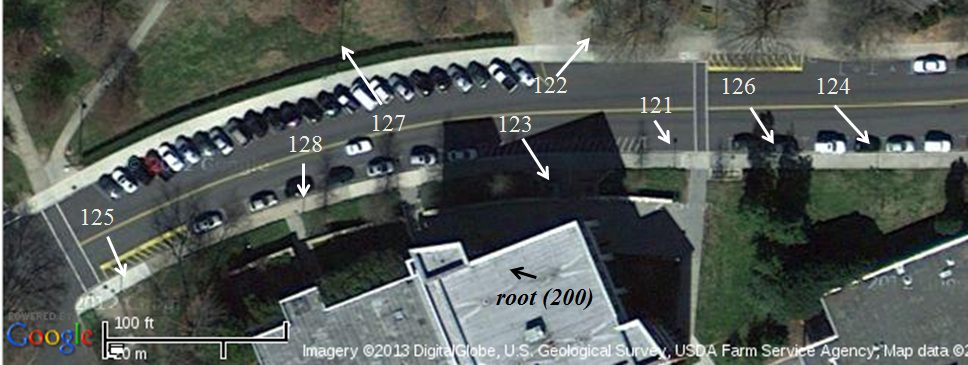
\includegraphics[width=\columnwidth]{img_deployment.png}
%\caption{Mote Deployment}
%\label{img_deployment}
%\end{figure}
%
%\begin{figure}[htbp]
%\centering
%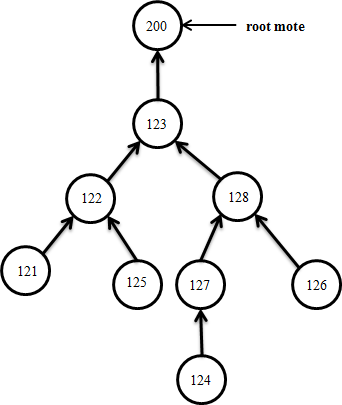
\includegraphics[width=8cm]{network.png}
%\caption{Observed Routing Topology}
%\label{img_network}
%\end{figure}
%
%In this section, we evaluate the reliability of the network based on two parameters: the percentage error in packet reception, and the ability of the network to tolerate mote failure.
%%, and the ability to eliminate partition of network.
% To evaluate these parameters we deployed eight motes on the lamp posts in front of Clemson University's School of Computing. The \textit{\textbf{root}} mote was deployed inside the School of Computing, as shown in Figure \ref{img_deployment}. The \textit{\textbf{root}} mote was connected to a desktop server process and periodically received data from the deployed motes. Figure \ref{img_network} shows the observed routing topology formed by the deployed motes.
%
%\subsection{Percentage Error in Packet Reception}\label{sec:percentage_error}
%In this subsection, we evaluate the percentage error in packet reception for each mote in the network. The percentage error in packet reception is defined as the ratio of the difference between the number of packets transmitted by the mote and the number of packets received at the base station, to the number of packets transmitted. That is, we consider end-to-end packet reception. To evaluate the percentage error in packet reception, we allowed the deployed motes to run continuously for 7 days. Each data packet sent by a mote to its parent contained a count of the total number of tries it took to successfully send the message, as well as the message number of the data being transferred. Table \ref{table_dataTransmitted} shows the total number of packets transmitted, the total number of packets received, the percentage error in packet reception, and the total number of tries before successful transmission of the packets over a period of 7 days.
%%To evaluate the yield of the network we deployed eight motes on the light polls in front of School of Computing, Clemson University, and the \textit{\textbf{root}} mote is deployed inside School of Computing. The \textit{\textbf{root}} mote is connected to the field deployed server and periodically receives data from the deployed motes. The deployed motes are (some (suggestion)) meters apart.
%%The data packet sent by the motes contains the number of tries by the mote before the parent mote received that packet and the count of message it transferred to the parent mote. We also calculate the error in packet reception for each mote. We maintain the count of packets received from each mote at the base station.
%
%
%\begin{table}[htbp]
%\begin{center}
%\begin{tabular}{|c|c|c|c|c|}
%\hline 
%\textbf{Mote} & \textbf{Count of} & \textbf{Count of} & \textbf{Percentage error} & \textbf{Total number} \\ 
% &   \textbf{packets}   &  \textbf{packets}  & \textbf{in packet} & \textbf{of retries}\\
% & \textbf{transmitted}  & \textbf{received} & \textbf{reception} & \\
%\hline  
%\hline  
%121 & 8714 & 8714 & 0 & 122 \\ 
%\hline 
%122 & 9047 & 9047 & 0 & 344 \\  
%\hline 
%123 & 10152 & 10152 & 0 & 4 \\ 
%\hline 
%124 & 8129 & 8129 & 0 & 161 \\ 
%\hline 
%125 & 9282 & 9282 & 0 & 165 \\ 
%\hline 
%126 & 6240 & 6240 & 0 & 184 \\  
%\hline 
%127 & 9182 & 9182 & 0 & 64 \\ 
%\hline 
%128 & 5195 & 5195 & 0 & 389 \\ 
%\hline 
%\hline
%\textbf{Total} & 65941 & 65941 & 0 & 1433 \\
%\hline
%\end{tabular}
%\end{center}
%\caption{Data Transmission Metrics}
%\label{table_dataTransmitted}
%\end{table}
%
%As we can see from Table \ref{table_dataTransmitted}, the percentage error in packet reception is 0. The packets transmitted by each mote are received at the base station. That is, the network achieved 100\% data yield. The number of retries before successful transmission of a data packet is less than 3\% of the total packets transmitted by all motes.
%
%%To check the reliability of the network when there are lots of packets in network we ran the same test as above with one extra mote in the network which constantly broadcast a packet of data every 10 milli second to make the network congested, during that scenario the error rate is less than one percent.
%
%\subsection{Ability to Tolerate Mote Failure}\label{sec:tolerate_mote_failure}
%In this subsection, we evaluate the ability of the network to withstand mote failures. To evaluate this property of the network, we followed the same experimental setup described in sections \ref{sec:reliability} and \ref{sec:percentage_error}. Figure \ref{img_network} shows the observed routing topology formed by the deployed motes. To evaluate the ability of the network to withstand mote failure, we introduced a fault by deactivating mote 128. Due to this, motes 127, 126, and 124 were disconnected from the network. We observed that motes 127, 126, and 124 detected the failure of mote 128, and rejoined the network, choosing another parent.
%% We can see from Tables \ref{table_selfHealingSystem} and \ref{table_selfHealingMote}, all of the failed motes rejoined the network.
%
%Regular (i.e., real) failure cases were also considered. Here, failure is defined as the removal of the mote from the network due to an obstruction between motes, an out of range mote, power failure, or a mote in the process of resetting. To determine the failure of the mote, we monitor the data received at the base station and timestamp the data. If the data is not received from a particular mote for 5 minutes then the mote is declared as failed. After that, whenever data is received from the failed mote, we conclude that the mote rejoined the network. Table \ref{table_selfHealingSystem} shows, over a period of a day, the number of mote failures recorded,  the number of rejoins that occurred within 10 minutes, and the number of failures that persisted beyond 10 minutes. Table \ref{table_selfHealingMote} shows, for each mote, over a period of 7 days, the number of failures the mote experienced, the number of times the mote was able to rejoin the network after a failure, and the number of times the mote was unable to rejoin the network after a failure. These figures suggest that the network is able to withstand mote failure.
%% To evaluate the self-healing property of the network we deployed eight motes on the light polls in front of School of Computing, Clemson University, and the \textit{\textbf{root}} mote is deployed inside School of Computing. The \textit{\textbf{root}} mote is connected to the field deployed server and periodically receives data from the deployed motes. The deployed motes are (some (suggestion)) meters apart.To evaluate the self-healing property of the network, we kept the deployed motes running continuously for 7 days. The data packet sent by the motes contains the number of tries by the mote before the parent mote received that packet and the count of message it transferred to the parent mote. Table \ref{table_selfHealingSystem} shows the number of motes failed, number of motes recovered, and number of motes unable to recover within 10 minutes each day on the system level. Table \ref{table_selfHealingMote} shows the number of failures, number of recoveries, and number of times unable to recover for each mote over a period of 7 days.
%
%\begin{table}[htbp]
%\begin{center}
%\begin{tabular}{|c|c|c|c|}
%\hline 
%\textbf{Day} & \textbf{Number of mote} & \textbf{Number of failures} & \textbf{Failures not} \\ 
% & \textbf{failures} & \textbf{corrected within} & \textbf{corrected within} \\ 
% &   & \textbf{10 minutes}  & \textbf{10 minutes} \\
%\hline 
%\hline 
%June 20 & 4 & 4 & 0 \\ 
%\hline 
%June 21 & 48 & 48 & 0 \\ 
%\hline 
%June 22 & 56 & 55 & 1 \\ 
%\hline 
%June 23 & 42 & 40 & 2 \\ 
%\hline 
%June 24 & 61 & 61 & 0 \\ 
%\hline 
%June 26 & 29 & 29 & 0 \\ 
%\hline 
%June 27 & 18 & 18 & 0 \\ 
%\hline 
%\end{tabular}
%\end{center} 
%\caption{Mote Failure Statistics (per day)}
%\label{table_selfHealingSystem}
%\end{table}
%
%
%\begin{table}[htbp]
%\begin{center}
%\begin{tabular}{|c|c|c|c|}
%\hline 
%\textbf{Mote} & \textbf{Number of} & \textbf{Number of failures} & \textbf{Failures not} \\ 
% & \textbf{failures} & \textbf{corrected within} & \textbf{corrected within} \\ 
% &   & \textbf{10 minutes}  & \textbf{10 minutes} \\
%\hline 
%\hline 
%121 & 7 & 7 & 0 \\ 
%\hline 
%122 & 9 & 9 & 0 \\ 
%\hline 
%123 & 0 & 0 & 0 \\ 
%\hline 
%124 & 9 & 9 & 0 \\ 
%\hline 
%125 & 9 & 9 & 0 \\ 
%\hline 
%126 & 38 & 38 & 0 \\ 
%\hline 
%127 & 5 & 5 & 0 \\ 
%\hline 
%128 & 181 & 178 & 3 \\ 
%\hline 
%\end{tabular}
%\end{center} 
%\caption{Mote Failure Statistics (per mote)}
%\label{table_selfHealingMote}
%\end{table}
%
%Table \ref{table_selfHealingSystem} shows that one mote was unable to recover on June 22, and two motes were unable to recover on June 23. We can see from Table \ref{table_selfHealingMote} that the only mote that was unable to recover is mote 128. The failure of mote 128 was purposefully introduced by disconnecting the battery. We can see from Tables \ref{table_selfHealingSystem} and \ref{table_selfHealingMote} that every other mote eventually recovered and rejoined the network within 10 minutes after failing. This supports our claims that the network is able to withstand mote failures.
%
%%\subsection{Partition-free Network} 
%%If a mote fails it divides the network in two subsets. In this subsection we evaluate our system and show that it is partition-free i.e. it prevents the network from partitioning. To evaluate the partition-free property of the network, we allowed the deployed motes to run continuously for 7 days. Each data packet, sent by a mote to its parent, contains a count of the total number of tries it took to successfully send the message, as well as the message number being transferred. Table \ref{table_partitionFreeSystem} shows the number of motes failed, number of motes recovered, and number of motes unable to recover each day.
%
%%To evaluate the partition property of the network, we kept the deployed motes running continuously for 7 days. The data packet sent by the motes contains the number of tries by the mote before the parent mote received that packet and the count of message it transferred to the parent mote. Table \ref{table_partitionFreeSystem} shows the number of motes failed, number of motes recovered, and number of motes unable to recover each day.
%
%%\begin{table}[htbp]
%%\begin{center}
%%\begin{tabular}{|c|c|c|c|}
%%\hline 
%%\textbf{Day} & \textbf{Number of motes} & \textbf{Number of motes} & \textbf{Number of motes} \\ 
%% & \textbf{Failed} & \textbf{recovered} & \textbf{unable to recover} \\ 
%%\hline 
%%\hline 
%%• & • & • & • \\ 
%%\hline 
%%• & • & • & • \\ 
%%\hline 
%%• & • & • & • \\ 
%%\hline 
%%• & • & • & • \\ 
%%\hline 
%%• & • & • & • \\ 
%%\hline 
%%• & • & • & • \\ 
%%\hline 
%%• & • & • & • \\ 
%%\hline 
%%• & • & • & • \\ 
%%\hline 
%%\end{tabular}
%%\end{center} 
%%\caption{Partition-free System}
%%\label{table_partitionFreeSystem}
%%\end{table}
%
%
%%We can see from Table \ref{table_partitionFreeSystem} that every mote recovers after failing, and joins the original network, and does not form a new network. This proves that the network is partition-free.
%
%The results presented in sections \ref{sec:percentage_error} and \ref{sec:tolerate_mote_failure} support our claim that the network is reliable.
%
%\section{Scalability}
%This section evaluates the scalability of our system. In this context, scalability depends on the internal message buffer size, the number of transmission slots per mote, and the baud-rate of the transceiver.
%
%Internal buffer size is an important factor in the evaluation of network scalability. In the experiments discussed in the previous sections, the size of the internal message buffer is 255 bytes, and the size of a data packet is 7 bytes. The maximum number of motes allowed in each transmission slot of the \textit{\textbf{root}} mote in the network is equal to the number of message packets that can be accommodated in the internal message buffer. It is assumed that each mote transmits exactly one data packet.
%\begin{center}
%$number\ of\ motes\ =\ \dfrac{255}{7}\ =\ 36.43$
%\end{center}
%
%Since the \textit{root} mote immediately transmits all received data to the base station, the network can accommodate 36 motes \textit{per child} of the \textit{root} mote, assuming an internal buffer size of 255 bytes per mote and a message packet size of 7 bytes.
%
%The total number of motes that can be accommodated in a network, depends on the number of transmission slots per mote. In our system, the duration of each transmission slot is 3 seconds (calculated in Section \ref{sec:trans_slots}), and data is transmitted every 60 seconds. Therefore, the total number of transmission slots that can be present in each period is $\dfrac{60\ (second)}{3\ (second)}\ =\ 20\ slots$. The total number of motes that can be accommodated in our system is as follows:
%
%\begin{equation}
%T_{motes}\ = N_{slots}*N_{motes} 
%\end{equation}
%
%
%\begin{tabular}{lllp{10cm}}
%where, &   &   &   \\ 
%%\hline 
%  & $T_{motes}$  & = & the maximum number of motes that can be accommodated in the network \\ 
%%\hline 
%  & $N_{slots}$ & = & the maximum number of transmission slots in a transmission period \\ 
%%\hline 
%  & $N_{motes}$ & = & the maximum number of motes in each transmission slot of the \textit{\textbf{root}} mote \\ 
%\end{tabular} 
%%where,\\
%%$T_{motes}$ = the maximum number of motes that can be accommodated in the network\\
%%$N_{slots}$ = the maximum number of transmission slots in a transmission period\\
%%$N_{motes}$ = the maximum number of motes in each transmission slot of \textit{\textbf{root}} mote\\
%
%\begin{center}
%$T_{motes}\ =\ 20\ *\ 36\ =\ 720\ motes$.
%\end{center}
%
%The baud-rate of the transceiver is also an important factor in the scalability of the network. The baud-rate of the RFM12 transceiver is 57.6 Kbps. The number of bytes that can be transmitted in one transmission slot, i.e. 3 seconds, is as follows:
%\begin{center}
%$number\ of\ bytes\ =\ \dfrac{3*57600}{8}\ =\ 21600$
%\end{center}
%
%Now we calculate the maximum number of bytes that can be transmitted in 3 seconds. The equation is as follows: 
%
%\begin{equation}
%T_{max} = N_{motes}*D_{bytes}
%\end{equation}
%
%\begin{tabular}{lllp{10cm}}
%where, &   &   &   \\ 
%  & $T_{max}$  & = & the maximum number of bytes transmitted during each transmission \\ 
%  & $N_{motes}$ & = & the maximum number of motes in each transmission slot of the \textit{\textbf{root}} mote \\ 
%  & $D_{bytes}$ & = & the size of a data message, including packet overhead \\ 
%\end{tabular} 
%
%\begin{center}
%$T_{max}\ =\ 36\ *\ 12\ =\ 432\ bytes$
%\end{center}
%In our system, even if each mote sends its data 20 times, we transmit a maximum of 8640 bytes (432 * 20) in 3 seconds per mote. The radio can easily handle the transmitted data.% The maximum data that can be transmitted by 720 motes in a period of 60 second is 288000 bytes.
%
%The calculations for internal buffer size, number of transmission slots per mote, and baud-rate of the transceiver together show that given the buffer size of 255 bytes and a message packet size of 7 bytes, this network can scale to accommodate 720 motes. To increase the number of motes beyond 720, we must increase the internal message buffer size.
%
%
%\section{Network Longevity}
%This section evaluates the longevity of the network. Here, network longevity is defined as the time period for which the network will work. The circuit operates both in the absence and presence of sunlight. We consider the lifetime of network in both cases.
%
%\subsection{Absence of Sunlight}\label{subsec:sunlight_absent}
%This subsection considers the lifetime of the network running only on battery power, in the absence of sunlight. Table \ref{table_powerConsumption} shows the power consumption of the microcontroller and the RFM12 transceiver in the active and sleep states.
%\begin{table}[htbp]
%\begin{center}
%\begin{tabular}{|c|c|c|c|}
%\hline 
%   & \textbf{Micro-} & \textbf{RFM12} & \textbf{Total} \\ 
%  &  \textbf{controller} &  &   \\ 
%\hline 
%\hline 
%\textbf{active} & 4.00 & 9.00 & 13.00 + $\alpha_{1}$ \\ 
%\hline 
%\textbf{sleep} & 0.52 & 0.10 & 0.62 + $\alpha_{2}$ \\ 
%\hline 
%\end{tabular}
%\end{center} 
%\caption{Device Current Consumption ($milliamps$)}
%\label{table_powerConsumption}
%\end{table}
%
%Our system works at a 10\% duty cycle; the motes transmit data every 60 seconds. Within a 60 second timeframe, the motes are in the active state for 6 seconds, and in the sleep state for 54 seconds (assumed each mote has maximum 2 children). The current consumption is calculated using the following formula:
%\begin{equation} \label{equ:current_consumption}
%C = \frac{A*on\ time + S*off\ time}{total\ time}
%\end{equation}
%%where,\\
%%C = Current consumption in $\ milliAmps$\\
%%A = Active state power consumption\\
%%S = Sleep state power consumption\\
%
%\begin{tabular}{lllp{10cm}}
%where, & • & • & • \\ 
%• & C & = & Current consumption in $\ milliamps$ \\ 
%• & A & = & Active state current consumption in $\ milliamps$ \\ 
%• & S & = & Sleep state current consumption in $\ milliamps$ \\ 
%\end{tabular} 
%
%\begin{center}
%$C = \dfrac{6*13.00 + 54*0.62}{60} = 1.858 \ milliamps$
%\end{center}
%The lifetime of a mote is calculated using the following formula:
%\begin{equation}
%Lifetime = \frac{Battery\ Capacity*0.80}{Current\ Consumption}
%\end{equation}
%The 0.80 in the equation indicates that we can use up to 80\% of the battery to run the circuit.
%\begin{center}
%$Lifetime\ =\ \dfrac{850*0.80}{1.858}\ =\ 365.98\ hrs\ =\ 15.25\ days$\\
%\end{center}
%
%The above calculation indicates that the network can run on battery power, in the absence of sunlight, for a period of 15.25 days.
%
%\subsection{Presence of Sunlight}\label{subsec:sunlight_present}
%This subsection evaluates the lifetime of the network running in the presence of sunlight. The solar panel generates 89 milliamps of current, and a voltage of 5 volts. Of the 89 milliamps of current, the solar panel supplies 17 milliamps of current to the processing circuit, and it supplies 50 milliamps of current to charge the Li-Ion battery. The remaining 12 milliamps of current is not used.
%
%As calculated in equation \ref{equ:current_consumption}, the mote consumes 1.858 milliamps of current. Let us assume that sunlight is available for 6 hours each day. As stated above, the solar panel will charge the battery by 6 * 50 = 300 mAh (best case charging). Each day, circuit runs on the battery for 18 hours. The power consumption from the battery is 18 * 1.858 = 33.44 mAh. As we can see, energy consumed is just 11.148 \% of the energy stored each day.
%
%The above calculations in subsections \ref{subsec:sunlight_absent} and \ref{subsec:sunlight_present} support our claim that the network will function properly for long periods without changing the batteries.
%\newpage
%--------------------------------------------------------------------------------------


%To evaluate this hardware and software solution we created ten motes. The mote as shown in Figure %\ref{img_prototypeBoard} consists of solar power circuit, battery circuit, switching circuit, and processing circuit.

%To test that the network is forming correctly, is reliable, partition free, and scalable, we setup the experiment in \textit{Dependable Systems Research Group} lab, \textit{Clemson University}. We deployed seven motes in the lab at different locations. In this experiment the motes were connected to fixed power supply.

%To test the working of solar power circuit, we placed three motes outside in sunlight.

%We placed the mote with Root status in lab, this mote is connected to the base station. The base station records the data and the number of packets received. The id of the mote with status Root is 200 and the id of other motes ranges from 101 to 109.

%[Note: The networks are dynamically formed when this program is used, for simplicity all the images of the network below are of same type, means the location of motes are fixed in the images]

%\section{Network formation}

%\begin{figure}
%\centering
%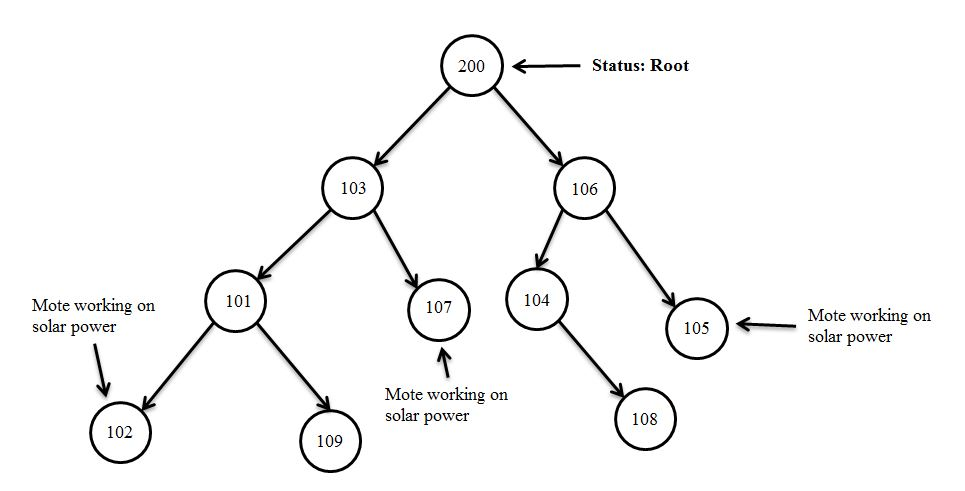
\includegraphics[width=\columnwidth]{network.JPG}
%\caption{Network formed}
%\label{img_network}
%\end{figure}

%In this experiment the mote with status of Root (id 200) is connected to the base station. The other motes when they wake up has status of idle. As discussed in section 3.2 they perform operations 1, 2, 3, 4, and 5 and forms the network. 
%The network formed by these motes is shown in Figure \ref{img_network}. All of the motes from id 101 to 109 tries to connect to the Root but only motes with id 103 and 106 succeeds in connecting with the mote id 200 in the first try. Now as mote with id 200 don't have any slots available, the other motes cannot join it. Whenever motes with id 103 and 106 get time synchronized with their parent the remaining motes can join them. This process is repeated until all the motes in idle state join the network.


%\section{Scalable}

%\begin{figure}
%\centering
%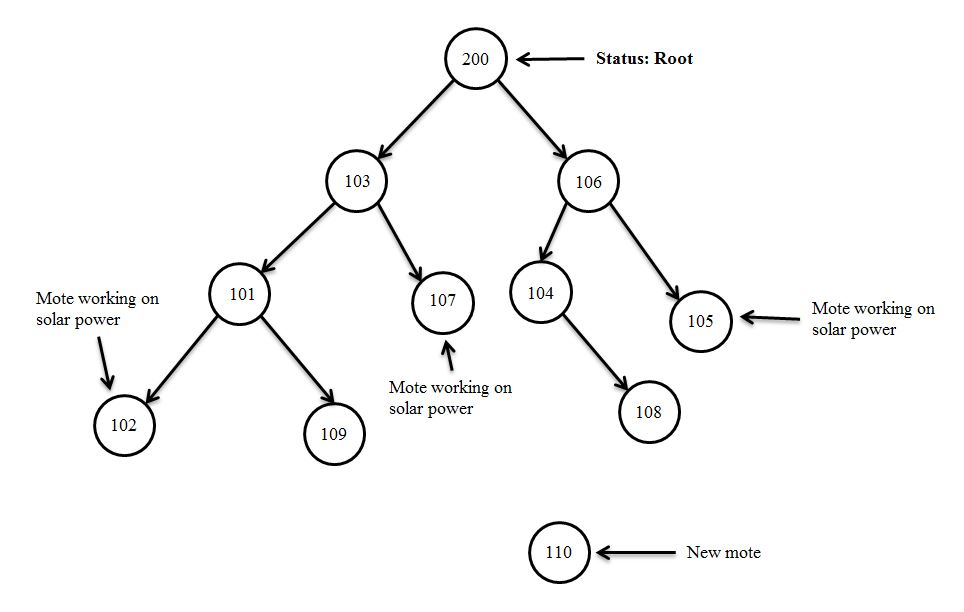
\includegraphics[width=\columnwidth]{network1.JPG}
%\caption{Scalable network}
%\label{img_network1}
%\end{figure}
%As shown in Figure \ref{img_network1}, if new mote (mote id 110 as indicated in Figure \ref{img_network1}) wants to join the  network. It performs operation 1 as discussed in section 3.2, If there is mote awake at that time and has free time slot available then operations 2, 3, 4, and 5 takes place and the new mote joins the network.

%To check the scalability function of the network, instead of waking all the motes at the same time, we wake up one mote at a time. We added nine motes using this technique and all the motes joined the network. This shows that the network formed using this software is scalable.


%\section{Partition free}

%\begin{figure}
%\centering
%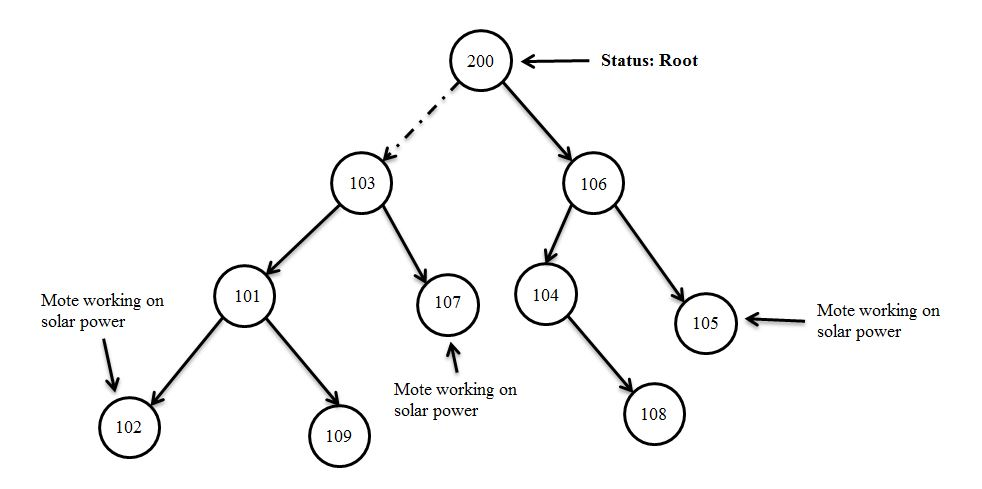
\includegraphics[width=\columnwidth]{network2.JPG}
%\caption{Partition free network}
%\label{img_network2}
%\end{figure}

%To evaluate that the network cannot remain partitioned for a longer period of time, as shown in Figure \ref{img_network2} we deliberately broke the link between mote id 200 and mote id 103 by changing the address of the parent of the mote id 103. This caused the network to break in two parts, one part consisting of mote id 200 as the Root mote and other part consisting of mote id 103 as the root mote. As a result of this scenario  mote id 103 stopped receiving synchronization signal. As the status of mote id 103 is Node it recognized this situation as the death of its parent. After detecting the death of the parent, mote id 103 propagated this death to is child and killed itself. All the motes connected to mote 103 killed themselves on reciving this signal as a result of operation 8 as discussed in section 3.2 . In the next step they again joined the network as new motes. This solved the problem of partition in the network.

%\section{Self healing}To evaluate the self healing property of the network, we intentionally killed mote 103, the already formed network is as shown in Figure \ref{img_network}. As a result of this motes 101 and 107 stopped receiving the synchronization signal, because of this they detected the death of their parent. Motes 101 and 107 then propagated the death to their child. After this the motes killed themselves. As discussed in section 3.2 Operation 8 takes place on the child motes and they also propagate the death to their child and killed themselves.